% Options for packages loaded elsewhere
\PassOptionsToPackage{unicode}{hyperref}
\PassOptionsToPackage{hyphens}{url}
%
\documentclass[
  ignorenonframetext,
]{beamer}
\title{Explorative Faktorenanalyse}
\author{Jalynskij et al.}
\date{}

\usepackage{pgfpages}
\setbeamertemplate{caption}[numbered]
\setbeamertemplate{caption label separator}{: }
\setbeamercolor{caption name}{fg=normal text.fg}
\beamertemplatenavigationsymbolsempty
% Prevent slide breaks in the middle of a paragraph
\widowpenalties 1 10000
\raggedbottom
\setbeamertemplate{part page}{
  \centering
  \begin{beamercolorbox}[sep=16pt,center]{part title}
    \usebeamerfont{part title}\insertpart\par
  \end{beamercolorbox}
}
\setbeamertemplate{section page}{
  \centering
  \begin{beamercolorbox}[sep=12pt,center]{part title}
    \usebeamerfont{section title}\insertsection\par
  \end{beamercolorbox}
}
\setbeamertemplate{subsection page}{
  \centering
  \begin{beamercolorbox}[sep=8pt,center]{part title}
    \usebeamerfont{subsection title}\insertsubsection\par
  \end{beamercolorbox}
}
\AtBeginPart{
  \frame{\partpage}
}
\AtBeginSection{
  \ifbibliography
  \else
    \frame{\sectionpage}
  \fi
}
\AtBeginSubsection{
  \frame{\subsectionpage}
}
\usepackage{amsmath,amssymb}
\usepackage{lmodern}
\usepackage{iftex}
\ifPDFTeX
  \usepackage[T1]{fontenc}
  \usepackage[utf8]{inputenc}
  \usepackage{textcomp} % provide euro and other symbols
\else % if luatex or xetex
  \usepackage{unicode-math}
  \defaultfontfeatures{Scale=MatchLowercase}
  \defaultfontfeatures[\rmfamily]{Ligatures=TeX,Scale=1}
\fi
\usetheme[]{Boadilla}
% Use upquote if available, for straight quotes in verbatim environments
\IfFileExists{upquote.sty}{\usepackage{upquote}}{}
\IfFileExists{microtype.sty}{% use microtype if available
  \usepackage[]{microtype}
  \UseMicrotypeSet[protrusion]{basicmath} % disable protrusion for tt fonts
}{}
\makeatletter
\@ifundefined{KOMAClassName}{% if non-KOMA class
  \IfFileExists{parskip.sty}{%
    \usepackage{parskip}
  }{% else
    \setlength{\parindent}{0pt}
    \setlength{\parskip}{6pt plus 2pt minus 1pt}}
}{% if KOMA class
  \KOMAoptions{parskip=half}}
\makeatother
\usepackage{xcolor}
\IfFileExists{xurl.sty}{\usepackage{xurl}}{} % add URL line breaks if available
\IfFileExists{bookmark.sty}{\usepackage{bookmark}}{\usepackage{hyperref}}
\hypersetup{
  pdftitle={Explorative Faktorenanalyse},
  pdfauthor={Jalynskij et al.},
  hidelinks,
  pdfcreator={LaTeX via pandoc}}
\urlstyle{same} % disable monospaced font for URLs
\newif\ifbibliography
\usepackage{color}
\usepackage{fancyvrb}
\newcommand{\VerbBar}{|}
\newcommand{\VERB}{\Verb[commandchars=\\\{\}]}
\DefineVerbatimEnvironment{Highlighting}{Verbatim}{commandchars=\\\{\}}
% Add ',fontsize=\small' for more characters per line
\usepackage{framed}
\definecolor{shadecolor}{RGB}{248,248,248}
\newenvironment{Shaded}{\begin{snugshade}}{\end{snugshade}}
\newcommand{\AlertTok}[1]{\textcolor[rgb]{0.94,0.16,0.16}{#1}}
\newcommand{\AnnotationTok}[1]{\textcolor[rgb]{0.56,0.35,0.01}{\textbf{\textit{#1}}}}
\newcommand{\AttributeTok}[1]{\textcolor[rgb]{0.77,0.63,0.00}{#1}}
\newcommand{\BaseNTok}[1]{\textcolor[rgb]{0.00,0.00,0.81}{#1}}
\newcommand{\BuiltInTok}[1]{#1}
\newcommand{\CharTok}[1]{\textcolor[rgb]{0.31,0.60,0.02}{#1}}
\newcommand{\CommentTok}[1]{\textcolor[rgb]{0.56,0.35,0.01}{\textit{#1}}}
\newcommand{\CommentVarTok}[1]{\textcolor[rgb]{0.56,0.35,0.01}{\textbf{\textit{#1}}}}
\newcommand{\ConstantTok}[1]{\textcolor[rgb]{0.00,0.00,0.00}{#1}}
\newcommand{\ControlFlowTok}[1]{\textcolor[rgb]{0.13,0.29,0.53}{\textbf{#1}}}
\newcommand{\DataTypeTok}[1]{\textcolor[rgb]{0.13,0.29,0.53}{#1}}
\newcommand{\DecValTok}[1]{\textcolor[rgb]{0.00,0.00,0.81}{#1}}
\newcommand{\DocumentationTok}[1]{\textcolor[rgb]{0.56,0.35,0.01}{\textbf{\textit{#1}}}}
\newcommand{\ErrorTok}[1]{\textcolor[rgb]{0.64,0.00,0.00}{\textbf{#1}}}
\newcommand{\ExtensionTok}[1]{#1}
\newcommand{\FloatTok}[1]{\textcolor[rgb]{0.00,0.00,0.81}{#1}}
\newcommand{\FunctionTok}[1]{\textcolor[rgb]{0.00,0.00,0.00}{#1}}
\newcommand{\ImportTok}[1]{#1}
\newcommand{\InformationTok}[1]{\textcolor[rgb]{0.56,0.35,0.01}{\textbf{\textit{#1}}}}
\newcommand{\KeywordTok}[1]{\textcolor[rgb]{0.13,0.29,0.53}{\textbf{#1}}}
\newcommand{\NormalTok}[1]{#1}
\newcommand{\OperatorTok}[1]{\textcolor[rgb]{0.81,0.36,0.00}{\textbf{#1}}}
\newcommand{\OtherTok}[1]{\textcolor[rgb]{0.56,0.35,0.01}{#1}}
\newcommand{\PreprocessorTok}[1]{\textcolor[rgb]{0.56,0.35,0.01}{\textit{#1}}}
\newcommand{\RegionMarkerTok}[1]{#1}
\newcommand{\SpecialCharTok}[1]{\textcolor[rgb]{0.00,0.00,0.00}{#1}}
\newcommand{\SpecialStringTok}[1]{\textcolor[rgb]{0.31,0.60,0.02}{#1}}
\newcommand{\StringTok}[1]{\textcolor[rgb]{0.31,0.60,0.02}{#1}}
\newcommand{\VariableTok}[1]{\textcolor[rgb]{0.00,0.00,0.00}{#1}}
\newcommand{\VerbatimStringTok}[1]{\textcolor[rgb]{0.31,0.60,0.02}{#1}}
\newcommand{\WarningTok}[1]{\textcolor[rgb]{0.56,0.35,0.01}{\textbf{\textit{#1}}}}
\usepackage{graphicx}
\makeatletter
\def\maxwidth{\ifdim\Gin@nat@width>\linewidth\linewidth\else\Gin@nat@width\fi}
\def\maxheight{\ifdim\Gin@nat@height>\textheight\textheight\else\Gin@nat@height\fi}
\makeatother
% Scale images if necessary, so that they will not overflow the page
% margins by default, and it is still possible to overwrite the defaults
% using explicit options in \includegraphics[width, height, ...]{}
\setkeys{Gin}{width=\maxwidth,height=\maxheight,keepaspectratio}
% Set default figure placement to htbp
\makeatletter
\def\fps@figure{htbp}
\makeatother
\setlength{\emergencystretch}{3em} % prevent overfull lines
\providecommand{\tightlist}{%
  \setlength{\itemsep}{0pt}\setlength{\parskip}{0pt}}
\setcounter{secnumdepth}{-\maxdimen} % remove section numbering
\ifLuaTeX
  \usepackage{selnolig}  % disable illegal ligatures
\fi

\begin{document}
\frame{\titlepage}

\begin{frame}{Einstieg}
\protect\hypertarget{einstieg}{}
\url{https://openpsychometrics.org/tests/IPIP-BFFM/1.php}
\end{frame}

\begin{frame}{Die ``Large Data Set Challenge''}
\protect\hypertarget{die-large-data-set-challenge}{}
\begin{example}
Stellen Sie sich vor, die von Ihnen soeben beantworteten Fragen ergäben die
Korrelationsmatrix $R$ auf der nächsten Folie. Die "Large Data Set Challenge"
lautet: Erkennen Sie eine Struktur in den Daten? D.h., wenn ja weiter; welche
Items könnten man Ihrer Meinung nach zu Itemgruppen zusammenfassen?
\end{example}

~

Anmerkung: Nein, das sind (wirklich) nicht ihre Antworten;
\(\texttt{V1 - V30}\) sind Zufallsvariablen!
\end{frame}

\begin{frame}[fragile]{Struktur erkennen \& Itemgruppen finden:
Übungsaufgabe 1}
\protect\hypertarget{struktur-erkennen-itemgruppen-finden-uxfcbungsaufgabe-1}{}
\begin{verbatim}
## Warning in sqrt(1 - diag(model)): NaNs produced
\end{verbatim}

\begin{center}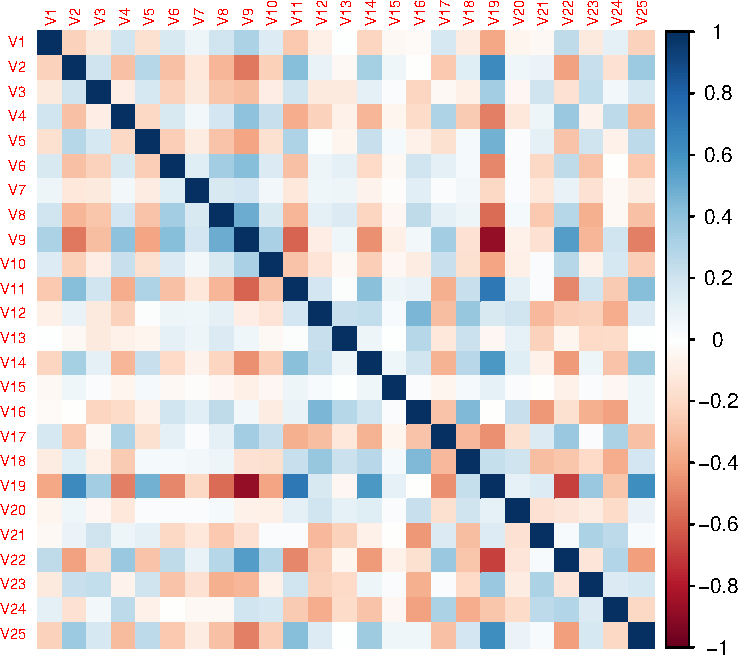
\includegraphics[width=0.7\linewidth]{06-EFA_files/figure-beamer/unnamed-chunk-1-1} \end{center}
\end{frame}

\begin{frame}{Die ``Large Data Set Challenge''}
\protect\hypertarget{die-large-data-set-challenge-1}{}
\begin{alertblock}{Large Data Set Challenge}
Mit zunehmender Itemzahl nimmt die wird die Anzahl der Korrelationen, die für
eine Analyse zu berücksichtigen sind schnell zu. Die "Challenge" ist eine
mögliche Struktur zu erkennen!
\end{alertblock}

In a Nutshell:

\begin{itemize}
\tightlist
\item
  Problem: Anzahl der Korrelationen
\item
  z.B.: \(25\) Items \(\widehat{=}\) \(2^{25} = 625\) Korrelationen
\item
  Krux: Struktur erkennen
\item
  \(\Leftrightarrow\) finde: hoch korrelierende Itemgruppen
\end{itemize}
\end{frame}

\begin{frame}{Explorative Faktorenanalyse: in a Nutshell}
\protect\hypertarget{explorative-faktorenanalyse-in-a-nutshell}{}
\begin{itemize}
\tightlist
\item
  (ein) Hilfsmittel: .. (explorative) \textbf{Faktorenanalyse}
\end{itemize}

~

\begin{block}{Faktorenanalyse}
"The basic idea is to find latent variables (factors) based on the correlation
structure of the manifest input variables (indicators)." (Mair 2018, S. 23)
\end{block}

\begin{itemize}
\item
  andere Helferlein zur \emph{Datenreduktion} (eine Auswahl):

  \begin{itemize}
  \tightlist
  \item
    Hauptkomponentenanalyse
  \item
    Clusteranalyse
  \item
    Explorative Likertskalierung
  \item
    (Non-) Metric Data Scaling (Voraus.: Distanzmatrizen)
  \end{itemize}
\end{itemize}

Wichtig: ``meaningful compression'' vs.~``full compression''
\end{frame}

\begin{frame}{Stategie \& Vorgehen: Simulieren \& Evaluieren}
\protect\hypertarget{stategie-vorgehen-simulieren-evaluieren}{}
\begin{enumerate}
\tightlist
\item
  Man erschaffe \(\geq 1\) eine latente Variable (LV)
\item
  \ldots lasse die LV Antwortmuster produzieren
\item
  \ldots wandel sie in eine Korrelationsmatrix um
\item
  \ldots und versucht die Struktur mit der Faktorenanalyse aufzufinden
\end{enumerate}

~

\begin{block}{Vom generativen Prozess zur Korrelationsmatrix}
Der generative Prozess, d.h. wie genau ein Konstrukt die Antworten auf den Items
erzeugt, bleibt meist verborgen. Wir untersuchen meistens lediglich
Verhaltensspuren des Konstruktes, die sich in den Items ausdrückt, d.h. in der
Struktur der Korrelationsmatrix niederschlägt. Strukturen zu simulieren ist
hilfreich, weil wir dort "die Wahrheit" kennen und das Verfahren damit besser
beurteilen können ($\sim$ fake data analysis)
\end{block}
\end{frame}

\begin{frame}[fragile]{``Playing Creator'': Zwei latente Variable
erschaffen}
\protect\hypertarget{playing-creator-zwei-latente-variable-erschaffen}{}
\begin{Shaded}
\begin{Highlighting}[]
\CommentTok{\# Anzahl der Items}
\NormalTok{N }\OtherTok{\textless{}{-}} \DecValTok{8}
\CommentTok{\# Faktorladungen}
\NormalTok{load\_F1 }\OtherTok{\textless{}{-}} \FunctionTok{c}\NormalTok{(}\FloatTok{0.6}\NormalTok{, }\SpecialCharTok{{-}}\FloatTok{0.3}\NormalTok{, }\FloatTok{0.5}\NormalTok{, }\FloatTok{0.7}\NormalTok{, }\FloatTok{0.1}\NormalTok{, }\FloatTok{0.2}\NormalTok{, }\FloatTok{0.2}\NormalTok{, }\FloatTok{0.3}\NormalTok{)}
\NormalTok{load\_F2 }\OtherTok{\textless{}{-}} \FunctionTok{c}\NormalTok{(}\SpecialCharTok{{-}}\FloatTok{0.1}\NormalTok{, }\FloatTok{0.1}\NormalTok{, }\FloatTok{0.1}\NormalTok{, }\FloatTok{0.1}\NormalTok{, }\SpecialCharTok{{-}}\FloatTok{0.7}\NormalTok{, }\FloatTok{0.5}\NormalTok{, }\SpecialCharTok{{-}}\FloatTok{0.6}\NormalTok{, }\FloatTok{0.7}\NormalTok{)}
\NormalTok{fx }\OtherTok{\textless{}{-}} \FunctionTok{cbind}\NormalTok{(load\_F1, load\_F2)}
\CommentTok{\# Zwischenfaktorkorrelation }
\NormalTok{phi }\OtherTok{\textless{}{-}} \FunctionTok{diag}\NormalTok{(}\FunctionTok{rep}\NormalTok{(}\DecValTok{1}\NormalTok{, }\DecValTok{2}\NormalTok{)) ; phi[}\DecValTok{1}\NormalTok{, }\DecValTok{2}\NormalTok{] }\OtherTok{\textless{}{-}}\NormalTok{ phi[}\DecValTok{2}\NormalTok{, }\DecValTok{1}\NormalTok{] }\OtherTok{\textless{}{-}} \FloatTok{0.6}
\CommentTok{\# Struktur }
\NormalTok{S }\OtherTok{\textless{}{-}}\NormalTok{ psych}\SpecialCharTok{::}\FunctionTok{sim.structure}\NormalTok{(fx, phi, }\AttributeTok{n=}\DecValTok{1000}\NormalTok{)}
\CommentTok{\# Korrelations{-} und Datenmatrix}
\NormalTok{R }\OtherTok{\textless{}{-}}\NormalTok{ S}\SpecialCharTok{$}\NormalTok{model ; X }\OtherTok{\textless{}{-}}\NormalTok{ S}\SpecialCharTok{$}\NormalTok{observed  }\CommentTok{\# R \textless{}{-} cor(X)}
\end{Highlighting}
\end{Shaded}
\end{frame}

\begin{frame}{Vom generativen Prozess zur Korrelationsmatrix}
\protect\hypertarget{vom-generativen-prozess-zur-korrelationsmatrix}{}
\end{frame}

\begin{frame}{Prognose \& Selbstexperiment: Übungsaufgabe 2}
\protect\hypertarget{prognose-selbstexperiment-uxfcbungsaufgabe-2}{}
\begin{example}
Versuchen Sie es selbst! Verändern sie systematisch $\texttt{F1; F2}$  und
$\texttt{phi}$.
1. Wie verändert sich die Korrelationsmatrix, in Abhängigkeiten
Ihrer Veränderungen? 
2. Können Sie eine eindeutige Struktur konstruieren? 
3. Wenn ja, mit welchen Werten von $\texttt{F1; F2}$  und $\texttt{phi}$ haben Sie ihr Ziel
erreicht?
\end{example}

\begin{example}
Haben Sie ein Strukturmodell gefunden, dass ihnen gefällt? Ja, dann überlegen
Sie sich jetzt für welche Konstrukte diese Struktur Sinn macht (z.B.:
extraversion $\sim$ openness to experience)
\end{example}
\end{frame}

\begin{frame}{Logik latenter Variablen (..reversed)}
\protect\hypertarget{logik-latenter-variablen-..reversed}{}
\begin{block}{Von der Korrelationsmatrix zur LV} Die Faktoranalyse
ist ein strukturentdeckendes Verfahren. D.h. den generativen Prozess, d.h. wie
ein Konstrukt die Antworten auf den Items verursacht hat anhand der Struktur die
sich in der vorgegebenen Korrelationsmatrix zu \textit{modellieren}.
\end{block}

\begin{itemize}
\tightlist
\item
  Modell: \emph{Common Factor Model} (CFM)
\end{itemize}

\begin{alertblock}{Eingangsgleichung}
  \begin{equation}
    x = \Lambda \xi + \epsilon
  \end{equation}
\end{alertblock}

~

\begin{quote}
``In other words EFA tries to find \(p\) latent variables on the basis
of the correlation structure of the \(m\) manifest variables.'' (ebd.)
\end{quote}
\end{frame}

\begin{frame}{Das Common Factor Model (CFM)}
\protect\hypertarget{das-common-factor-model-cfm}{}
Anmerkung: Für die Reformulierung von Gleichung (1) zu (2): siehe
\href{http://dx.doi.org/10.4135/9780857020994.n6}{McCallum (2009)}

\begin{alertblock}{Fudnamentaltheorem}
  \begin{equation}
    P = \Lambda \Phi \Lambda^{t} + \Psi
  \end{equation}
\end{alertblock}

\begin{itemize}
\tightlist
\item
  \(P\): Modell-implizierte Korrelationsmatrix
\item
  \(\Lambda\): Ladungsmatrix
\item
  \(\Phi\): Matrix der Zwischenfaktorkorrelationen
\item
  \(\Psi\): Uniqueness
\end{itemize}

\begin{block}{Zusammenhang: Modell \& Struktur}
Die von ihnen konstruierte Struktur versuchen wir nun mit der Faktorenanalyse
unter Einsatz des CFM zu rekonstruieren. Das CFM ist also Ihr Tool im
bevorstehenden Rekonstruktionsprozess!
\end{block}
\end{frame}

\begin{frame}{Fakotrenanalyse: ``A hurdle race''}
\protect\hypertarget{fakotrenanalyse-a-hurdle-race}{}
\begin{enumerate}
\tightlist
\item
  Hürde: Extraktionsproblem
\item
  Hürde: Rotationsproblem
\item
  Hürde: Problem der Anzahl zu extrahierender Faktoren
\end{enumerate}

~

\begin{quote}
``Unfortunately, factor analysis is frequently misunderstood and often
misused. Some researchers appear to use factor analysis as a kind of
divining rod, hoping to find gold hidden underneath tons of dirt. But
there is nothing magical about the technique. {[}\(\dots\){]} Factor
analysis will yield meaningful results only when the research was
meaningful to begin with.''
\href{https://www.pearson.com/us/higher-education/program/Gregory-Psychological-Testing-History-Principles-and-Applications-7th-Edition/PGM332874.html}{Gregory
(2014, S. 165)}
\end{quote}

Konklusion: Versuchen Sie ihr Modell zu verstehen!
\end{frame}

\begin{frame}{Extraktionsproblem}
\protect\hypertarget{extraktionsproblem}{}
\begin{alertblock}{Extraktionsproblem}
  Wie extrahieren wir die Faktoren/Komponenten 
\end{alertblock}

\begin{enumerate}
\tightlist
\item
  Lösung: Bestimmung der ``Principal Components''

  \begin{itemize}
  \tightlist
  \item
    Verfahren: PCA (Principal Component Analysis/Method)
  \item
    Modellgleichung: \(R \leftarrow P = CC^{t}\)
  \item
    Note: Eigenwert-, Singulärwertzerlegung (closed form solution)
  \end{itemize}
\item
  Lösung: Iterative Bestimmung der ``Principal Components''

  \begin{itemize}
  \tightlist
  \item
    Verfahren: PAFA (Principal Axis Factor Analysis)
  \item
    Modellgleichung: \(R^* \leftarrow P = FF^{t}\)
  \item
    Note(s): Reduzierte Matrix, iterativer Prozess (convergence issues)
  \end{itemize}
\item
  Lösung: Finde die plausibelsten (``most likely'') Werte zur Repro

  \begin{itemize}
  \tightlist
  \item
    Verfahren: MLFA (Maximum Likelihood Factor Analysis)
  \item
    Modellgleichung:
    \(R \leftarrow P = \Lambda \Phi \Lambda^{t} + \Psi\)
  \item
    Note(s): Reduzierte Matrix, itterativer Prozess (convergence issues)
  \end{itemize}
\end{enumerate}
\end{frame}

\begin{frame}[fragile]{Hauptkomponentenanalyse}
\protect\hypertarget{hauptkomponentenanalyse}{}
Ziel: Maximale (Gesamt-)Varianzaufklärung; d.h: minimaler
Informationsverlust

~

\begin{Shaded}
\begin{Highlighting}[]
\CommentTok{\# Old School!}
\NormalTok{(dino\_pca }\OtherTok{\textless{}{-}} \FunctionTok{princomp}\NormalTok{(X, }\AttributeTok{cor=}\ConstantTok{TRUE}\NormalTok{))}
\CommentTok{\# New School}
\NormalTok{pca\_fit }\OtherTok{\textless{}{-}}\NormalTok{ psych}\SpecialCharTok{::}\FunctionTok{principal}\NormalTok{(R, }\AttributeTok{nfactors =} \DecValTok{2}\NormalTok{, }
                            \AttributeTok{rotate =} \StringTok{"none"}\NormalTok{)}
\DocumentationTok{\#\# Komponentenladungen}
\NormalTok{pca\_fit}\SpecialCharTok{$}\NormalTok{loadings}
\DocumentationTok{\#\# Kommunalitäten }
\NormalTok{pca\_fit}\SpecialCharTok{$}\NormalTok{communality}
\DocumentationTok{\#\# Uniqueness }
\NormalTok{pca\_fit}\SpecialCharTok{$}\NormalTok{uniquenesses}
\end{Highlighting}
\end{Shaded}
\end{frame}

\begin{frame}{Übungsaufgabe 3: Selbstexperiment}
\protect\hypertarget{uxfcbungsaufgabe-3-selbstexperiment}{}
\begin{example}
Versuchen Sie es nun selbst! Fitten sie ein PC model. Interpretieren Sie die
enstprechenden Kennwerte für ihr Model und präsentieren Sie diese mir oder ihrem
Nachbarn. Verändern Sie auch einmal die Anzahl der zu extrahierenden Faktoren
($\texttt{nfactors}$). Wie verändert sich ihre Lösung wenn sie die Zahl
vergößern, bzw. verkleinern? Wie wirken sich diese Veränderungen auf die
Interpretation Ihrer Ergebnisse aus? 
\end{example}

Anmerkung: Denken Sie daran, normalerweise kennen Sie die Anzahl der zu
extrahierenden Komponenten/Faktoren nicht. Wie man dieses Problem
angeht, dazu gleich mehr!
\end{frame}

\begin{frame}[fragile]{Principal Axis Factor Analysis}
\protect\hypertarget{principal-axis-factor-analysis}{}
\begin{itemize}
\tightlist
\item
  Ziel: sukkzessive Varianzaufklärung der \emph{gemeinsamen} (nicht der
  Gesamt-) Varianz
\item
  Basis: \emph{reduzierte} Korrelationsmatrix (\(R^*\)).
\item
  Verständnisprobleme? (siehe v.a: Selbststudium 3)
\end{itemize}

\begin{verbatim}
## Warning: factor.pa is deprecated. Please use the fa function with fm=pa
\end{verbatim}

\begin{verbatim}
## Factor Analysis using method =  pa
## Call: psych::factor.pa(r = R, nfactors = 2, rotate = "none")
## Unstandardized loadings (pattern matrix) based upon covariance matrix
##      PA1   PA2    h2   u2    H2   U2
## V1  0.43  0.34 0.298 0.70 0.299 0.70
## V2 -0.17 -0.19 0.064 0.94 0.064 0.94
## V3  0.53  0.21 0.320 0.68 0.320 0.68
## V4  0.70  0.30 0.583 0.42 0.581 0.42
## V5 -0.55  0.33 0.417 0.58 0.418 0.58
## V6  0.63 -0.10 0.410 0.59 0.410 0.59
## V7 -0.38  0.34 0.256 0.74 0.257 0.74
## V8  0.90 -0.13 0.830 0.17 0.830 0.17
## 
##                        PA1  PA2
## SS loadings           2.64 0.53
## Proportion Var        0.33 0.07
## Cumulative Var        0.33 0.40
## Proportion Explained  0.83 0.17
## Cumulative Proportion 0.83 1.00
## 
##  Standardized loadings (pattern matrix)
##    item   PA1   PA2    h2   u2
## V1    1  0.43  0.34 0.299 0.70
## V2    2 -0.17 -0.19 0.064 0.94
## V3    3  0.53  0.21 0.320 0.68
## V4    4  0.70  0.30 0.581 0.42
## V5    5 -0.55  0.33 0.418 0.58
## V6    6  0.63 -0.10 0.410 0.59
## V7    7 -0.38  0.34 0.257 0.74
## V8    8  0.90 -0.13 0.830 0.17
## 
##                  PA1  PA2
## SS loadings     2.64 0.54
## Proportion Var  0.33 0.07
## Cumulative Var  0.33 0.40
## Cum. factor Var 0.83 1.00
## 
## Mean item complexity =  1.5
## Test of the hypothesis that 2 factors are sufficient.
## 
## The degrees of freedom for the null model are  28  and the objective function was  1.96
## The degrees of freedom for the model are 13  and the objective function was  0 
## 
## The root mean square of the residuals (RMSR) is  0 
## The df corrected root mean square of the residuals is  0 
## 
## Fit based upon off diagonal values = 1
## Measures of factor score adequacy             
##                                                    PA1   PA2
## Correlation of (regression) scores with factors   0.94  0.69
## Multiple R square of scores with factors          0.89  0.48
## Minimum correlation of possible factor scores     0.78 -0.04
\end{verbatim}
\end{frame}

\begin{frame}{Übungsaufgabe 4: Kritische Reflexion}
\protect\hypertarget{uxfcbungsaufgabe-4-kritische-reflexion}{}
\begin{example}
Eine Folge der Extraktion mittels mit der Hauptkomponentenmethode ist, dass die
extrahierten Faktoren unabhängig voneinander sind. Glauben Sie dem Modell
uneingeschränkt, nähmen sie damit implizit an, dass auch die zugrundeliegende
Konstrukte unabhängig voneinander sein müssten. Denken Sie an ihr Beispiel. Für
wie plausibel halten Sie diese Annahme? Diskutieren Sie (heftig)! 
\end{example}

Warnhinweis: Sollte ein Inferno entfachen, halten Sie bitte Fluchtwege
sowie Zugänge zu den Feuerlöschern frei!
\end{frame}

\begin{frame}{Maximum Likelihood Factor Analysis}
\protect\hypertarget{maximum-likelihood-factor-analysis}{}
\begin{quote}
``Assuming that the residual variance reflects normally distributed
random error, the most elegant statistical solution is that of maximum
likelihood'' (Revelle, in prep. S. 156)
\end{quote}

\begin{alertblock}{KOmmunalitätenproblem}
Das CFM ($\Lambda \Phi \Lambda' + \Psi$) ist unbestimmt. D.h. es hat (deutlich)
mehr unbekannte 

\end{alertblock}
\end{frame}

\begin{frame}{Rotationsproblem}
\protect\hypertarget{rotationsproblem}{}
\end{frame}

\begin{frame}{Orthogonale Rotation}
\protect\hypertarget{orthogonale-rotation}{}
\end{frame}

\begin{frame}{Oblique Rotation}
\protect\hypertarget{oblique-rotation}{}
\end{frame}

\begin{frame}{Problem der Anzahl zu extrahierender Faktoren}
\protect\hypertarget{problem-der-anzahl-zu-extrahierender-faktoren}{}
\end{frame}

\begin{frame}[fragile]{(Reduzierte) Korrelationsmatrix}
\protect\hypertarget{reduzierte-korrelationsmatrix}{}
\begin{verbatim}
## maximum iteration exceeded
\end{verbatim}

\begin{verbatim}
## Loading required namespace: GPArotation
\end{verbatim}

\begin{verbatim}
## maximum iteration exceeded
## maximum iteration exceeded
## maximum iteration exceeded
\end{verbatim}

\begin{verbatim}
## $`iteration 1`
##       V1    V2    V3    V4    V5    V6    V7    V8
## V1  0.27 -0.14  0.30  0.40 -0.13  0.24 -0.05  0.34
## V2 -0.14  0.07 -0.13 -0.18  0.03 -0.09  0.00 -0.13
## V3  0.30 -0.13  0.32  0.43 -0.22  0.31 -0.13  0.45
## V4  0.40 -0.18  0.43  0.52 -0.29  0.41 -0.16  0.59
## V5 -0.13  0.03 -0.22 -0.29  0.39 -0.38  0.32 -0.54
## V6  0.24 -0.09  0.31  0.41 -0.38  0.41 -0.27  0.58
## V7 -0.05  0.00 -0.13 -0.16  0.32 -0.27  0.24 -0.38
## V8  0.34 -0.13  0.45  0.59 -0.54  0.58 -0.38  0.74
## 
## $`iteration 2`
##       V1    V2    V3    V4    V5    V6    V7    V8
## V1  0.29 -0.14  0.30  0.40 -0.13  0.24 -0.05  0.34
## V2 -0.14  0.07 -0.13 -0.18  0.03 -0.09  0.00 -0.13
## V3  0.30 -0.13  0.33  0.43 -0.22  0.31 -0.13  0.45
## V4  0.40 -0.18  0.43  0.55 -0.29  0.41 -0.16  0.59
## V5 -0.13  0.03 -0.22 -0.29  0.41 -0.38  0.32 -0.54
## V6  0.24 -0.09  0.31  0.41 -0.38  0.42 -0.27  0.58
## V7 -0.05  0.00 -0.13 -0.16  0.32 -0.27  0.26 -0.38
## V8  0.34 -0.13  0.45  0.59 -0.54  0.58 -0.38  0.78
## 
## $`iteration 3`
##       V1    V2    V3    V4    V5    V6    V7    V8
## V1  0.30 -0.14  0.30  0.40 -0.13  0.24 -0.05  0.34
## V2 -0.14  0.07 -0.13 -0.18  0.03 -0.09  0.00 -0.13
## V3  0.30 -0.13  0.32  0.43 -0.22  0.31 -0.13  0.45
## V4  0.40 -0.18  0.43  0.57 -0.29  0.41 -0.16  0.59
## V5 -0.13  0.03 -0.22 -0.29  0.42 -0.38  0.32 -0.54
## V6  0.24 -0.09  0.31  0.41 -0.38  0.42 -0.27  0.58
## V7 -0.05  0.00 -0.13 -0.16  0.32 -0.27  0.26 -0.38
## V8  0.34 -0.13  0.45  0.59 -0.54  0.58 -0.38  0.81
## 
## $`iteration 4`
##       V1    V2    V3    V4    V5    V6    V7    V8
## V1  0.30 -0.14  0.30  0.40 -0.13  0.24 -0.05  0.34
## V2 -0.14  0.06 -0.13 -0.18  0.03 -0.09  0.00 -0.13
## V3  0.30 -0.13  0.32  0.43 -0.22  0.31 -0.13  0.45
## V4  0.40 -0.18  0.43  0.57 -0.29  0.41 -0.16  0.59
## V5 -0.13  0.03 -0.22 -0.29  0.42 -0.38  0.32 -0.54
## V6  0.24 -0.09  0.31  0.41 -0.38  0.41 -0.27  0.58
## V7 -0.05  0.00 -0.13 -0.16  0.32 -0.27  0.26 -0.38
## V8  0.34 -0.13  0.45  0.59 -0.54  0.58 -0.38  0.82
\end{verbatim}
\end{frame}

\begin{frame}{PCA}
\protect\hypertarget{pca}{}
\end{frame}

\begin{frame}{PAFA}
\protect\hypertarget{pafa}{}
\end{frame}

\begin{frame}{Exkurs}
\protect\hypertarget{exkurs}{}
\end{frame}

\begin{frame}{MLFA}
\protect\hypertarget{mlfa}{}
\begin{alertblock}{Kommunalitätenproblem}
  "The problem is that in order to estimate the communalities, we need the
  loadings. Conversely, in order to estimate the loadings, we need the
  communalities." (Mair 2018, S. 24)
\end{alertblock}
\end{frame}

\begin{frame}{Später}
\protect\hypertarget{spuxe4ter}{}
Findet die Faktorenanalyse ihre Struktur?

Vanishing effekt -- Simulation? Korrelationsmatrix (grafisch: Vanishing
effect) (1) Faktorenanalyse mit zunehmender Zwischenfaktorkorrelation
(2) Faktorenanalyse mit abnehmenden Ladungen
\end{frame}

\begin{frame}{Fakotrscores}
\protect\hypertarget{fakotrscores}{}
Man könnte versuchen mit den Faktorscores die True Scores der Probanden
vorherzusagen
\end{frame}

\begin{frame}{Zusatzmaterial: PCA versus EFA}
\protect\hypertarget{zusatzmaterial-pca-versus-efa}{}
\textbackslash begin\{block\}\{EFA = PCA\} EFA und PCA entsprechen sich,
genau dann wenn man beim berechnen der Kennwerte die Korrelationsmatrix,
nicht die reduzierte Korrelationsmatrix verwendet wird und man als
Extraktionsmethode eine Eigenwertzerlegung der Korrelationsmatrix bzw.
eine Singulärwertzerlegung der Datenmatrix durchführt.
\textbackslash end\{alertblock\}
\end{frame}

\begin{frame}[fragile]{Zusatzmaterial: die Relevanz von Iterationen}
\protect\hypertarget{zusatzmaterial-die-relevanz-von-iterationen}{}
\ldots bei der Anpassungsgüte des Modells in der PAFA

\begin{verbatim}
##  [1] 2.508165e-02 3.040011e-03 3.681981e-04 5.153387e-05 9.036700e-06
##  [6] 1.994291e-06 5.300246e-07 1.605099e-07 1.605099e-07 1.605099e-07
\end{verbatim}

\includegraphics{06-EFA_files/figure-beamer/unnamed-chunk-8-1.pdf}
\end{frame}

\begin{frame}{Selbststudium 1: händische PCA -- Eigenwertzerlegung}
\protect\hypertarget{selbststudium-1-huxe4ndische-pca-eigenwertzerlegung}{}
\end{frame}

\begin{frame}{Selbststudium 2: händische EFA -- Singulärwertzerlegung}
\protect\hypertarget{selbststudium-2-huxe4ndische-efa-singuluxe4rwertzerlegung}{}
\end{frame}

\begin{frame}{Selbststudium 3}
\protect\hypertarget{selbststudium-3}{}
\begin{quote}
\ldots{[}P{]}rincipal axes factor analysis. This is similar to principal
components, except that it is done with a reduced matrix where the
diagonals are the communalities. The communalities can either be (1)
specified a priori, (2) estimated by such procedures as multiple linear
regression, or (3) found by iteratively doing an eigenvalue
decomposition and repeatedly replacing the original 1s on the diagonal
with the the value of \(1 - u^2\) where \(U^2 = diag(R−FF')\). That is,
\end{quote}

\begin{itemize}
\tightlist
\item
  Hier: Sukkzessive Eigenwertzerlegung
\end{itemize}
\end{frame}

\begin{frame}[fragile]{Wie sieht eine reduzierte Korrelationsmatrix
aus?}
\protect\hypertarget{wie-sieht-eine-reduzierte-korrelationsmatrix-aus}{}
\ldots Der Output zeigt die erst 8 Iterationen einer PAFA. Vergleichen
Sie diese mit ihre am Anfang konstruierte Korrelationsmatrix
(\(\texttt{R}\)). Achten Sie auf die Hauptdiagonale!

\begin{verbatim}
## maximum iteration exceeded
## maximum iteration exceeded
## maximum iteration exceeded
## maximum iteration exceeded
## maximum iteration exceeded
## maximum iteration exceeded
## maximum iteration exceeded
## maximum iteration exceeded
\end{verbatim}

\begin{verbatim}
## $`iteration 1`
##       V1    V2    V3    V4    V5    V6    V7    V8
## V1  0.27 -0.14  0.30  0.40 -0.13  0.24 -0.05  0.34
## V2 -0.14  0.07 -0.13 -0.18  0.03 -0.09  0.00 -0.13
## V3  0.30 -0.13  0.32  0.43 -0.22  0.31 -0.13  0.45
## V4  0.40 -0.18  0.43  0.52 -0.29  0.41 -0.16  0.59
## V5 -0.13  0.03 -0.22 -0.29  0.39 -0.38  0.32 -0.54
## V6  0.24 -0.09  0.31  0.41 -0.38  0.41 -0.27  0.58
## V7 -0.05  0.00 -0.13 -0.16  0.32 -0.27  0.24 -0.38
## V8  0.34 -0.13  0.45  0.59 -0.54  0.58 -0.38  0.74
## 
## $`iteration 2`
##       V1    V2    V3    V4    V5    V6    V7    V8
## V1  0.29 -0.14  0.30  0.40 -0.13  0.24 -0.05  0.34
## V2 -0.14  0.07 -0.13 -0.18  0.03 -0.09  0.00 -0.13
## V3  0.30 -0.13  0.33  0.43 -0.22  0.31 -0.13  0.45
## V4  0.40 -0.18  0.43  0.55 -0.29  0.41 -0.16  0.59
## V5 -0.13  0.03 -0.22 -0.29  0.41 -0.38  0.32 -0.54
## V6  0.24 -0.09  0.31  0.41 -0.38  0.42 -0.27  0.58
## V7 -0.05  0.00 -0.13 -0.16  0.32 -0.27  0.26 -0.38
## V8  0.34 -0.13  0.45  0.59 -0.54  0.58 -0.38  0.78
## 
## $`iteration 3`
##       V1    V2    V3    V4    V5    V6    V7    V8
## V1  0.30 -0.14  0.30  0.40 -0.13  0.24 -0.05  0.34
## V2 -0.14  0.07 -0.13 -0.18  0.03 -0.09  0.00 -0.13
## V3  0.30 -0.13  0.32  0.43 -0.22  0.31 -0.13  0.45
## V4  0.40 -0.18  0.43  0.57 -0.29  0.41 -0.16  0.59
## V5 -0.13  0.03 -0.22 -0.29  0.42 -0.38  0.32 -0.54
## V6  0.24 -0.09  0.31  0.41 -0.38  0.42 -0.27  0.58
## V7 -0.05  0.00 -0.13 -0.16  0.32 -0.27  0.26 -0.38
## V8  0.34 -0.13  0.45  0.59 -0.54  0.58 -0.38  0.81
## 
## $`iteration 4`
##       V1    V2    V3    V4    V5    V6    V7    V8
## V1  0.30 -0.14  0.30  0.40 -0.13  0.24 -0.05  0.34
## V2 -0.14  0.06 -0.13 -0.18  0.03 -0.09  0.00 -0.13
## V3  0.30 -0.13  0.32  0.43 -0.22  0.31 -0.13  0.45
## V4  0.40 -0.18  0.43  0.57 -0.29  0.41 -0.16  0.59
## V5 -0.13  0.03 -0.22 -0.29  0.42 -0.38  0.32 -0.54
## V6  0.24 -0.09  0.31  0.41 -0.38  0.41 -0.27  0.58
## V7 -0.05  0.00 -0.13 -0.16  0.32 -0.27  0.26 -0.38
## V8  0.34 -0.13  0.45  0.59 -0.54  0.58 -0.38  0.82
## 
## $`iteration 5`
##       V1    V2    V3    V4    V5    V6    V7    V8
## V1  0.30 -0.14  0.30  0.40 -0.13  0.24 -0.05  0.34
## V2 -0.14  0.06 -0.13 -0.18  0.03 -0.09  0.00 -0.13
## V3  0.30 -0.13  0.32  0.43 -0.22  0.31 -0.13  0.45
## V4  0.40 -0.18  0.43  0.58 -0.29  0.41 -0.16  0.59
## V5 -0.13  0.03 -0.22 -0.29  0.42 -0.38  0.32 -0.54
## V6  0.24 -0.09  0.31  0.41 -0.38  0.41 -0.27  0.58
## V7 -0.05  0.00 -0.13 -0.16  0.32 -0.27  0.26 -0.38
## V8  0.34 -0.13  0.45  0.59 -0.54  0.58 -0.38  0.82
## 
## $`iteration 6`
##       V1    V2    V3    V4    V5    V6    V7    V8
## V1  0.30 -0.14  0.30  0.40 -0.13  0.24 -0.05  0.34
## V2 -0.14  0.06 -0.13 -0.18  0.03 -0.09  0.00 -0.13
## V3  0.30 -0.13  0.32  0.43 -0.22  0.31 -0.13  0.45
## V4  0.40 -0.18  0.43  0.58 -0.29  0.41 -0.16  0.59
## V5 -0.13  0.03 -0.22 -0.29  0.42 -0.38  0.32 -0.54
## V6  0.24 -0.09  0.31  0.41 -0.38  0.41 -0.27  0.58
## V7 -0.05  0.00 -0.13 -0.16  0.32 -0.27  0.26 -0.38
## V8  0.34 -0.13  0.45  0.59 -0.54  0.58 -0.38  0.83
## 
## $`iteration 7`
##       V1    V2    V3    V4    V5    V6    V7    V8
## V1  0.30 -0.14  0.30  0.40 -0.13  0.24 -0.05  0.34
## V2 -0.14  0.06 -0.13 -0.18  0.03 -0.09  0.00 -0.13
## V3  0.30 -0.13  0.32  0.43 -0.22  0.31 -0.13  0.45
## V4  0.40 -0.18  0.43  0.58 -0.29  0.41 -0.16  0.59
## V5 -0.13  0.03 -0.22 -0.29  0.42 -0.38  0.32 -0.54
## V6  0.24 -0.09  0.31  0.41 -0.38  0.41 -0.27  0.58
## V7 -0.05  0.00 -0.13 -0.16  0.32 -0.27  0.26 -0.38
## V8  0.34 -0.13  0.45  0.59 -0.54  0.58 -0.38  0.83
## 
## $`iteration 8`
##       V1    V2    V3    V4    V5    V6    V7    V8
## V1  0.30 -0.14  0.30  0.40 -0.13  0.24 -0.05  0.34
## V2 -0.14  0.06 -0.13 -0.18  0.03 -0.09  0.00 -0.13
## V3  0.30 -0.13  0.32  0.43 -0.22  0.31 -0.13  0.45
## V4  0.40 -0.18  0.43  0.58 -0.29  0.41 -0.16  0.59
## V5 -0.13  0.03 -0.22 -0.29  0.42 -0.38  0.32 -0.54
## V6  0.24 -0.09  0.31  0.41 -0.38  0.41 -0.27  0.58
## V7 -0.05  0.00 -0.13 -0.16  0.32 -0.27  0.26 -0.38
## V8  0.34 -0.13  0.45  0.59 -0.54  0.58 -0.38  0.83
\end{verbatim}
\end{frame}

\end{document}
